\section{Introduction}\label{sec:introduction}
The pursuit of performance optimization in the field of high-performance computing (HPC) continues to push boundaries, with significant emphasis being placed on mitigating the impact of the increasing processor-memory speed gap and the rising computational memory requirements. These challenges are amplified by the escalating complexity of modern programs, making it increasingly difficult for experts to form a mental model of a program's data movement, let alone domain researchers. These factors have led to a marked surge in the costs of data movement and the appearance of severe performance bottlenecks. While advancements in hardware can alleviate some of these issues, the software community must also step up to the challenge, enhancing data locality through software to optimize data movement and access.

In this context, this paper focuses on the visualization of data movements and accesses, an often overlooked yet critical aspect of understanding and optimizing the complex data behavior of modern programs. Through a detailed overview of various methods of data acquisition, including dynamic analysis, static analysis, and cache simulation, this paper aims to shed light on the intricate world of data movement. By discussing different visualizations at varying granularities, it seeks to arm performance engineers with the necessary tools to enhance a program's data locality.

This contribution stands out as it provides a consolidated overview of different data visualization methods, enabling practitioners to select and employ the most suitable ones based on their specific needs and the complexity of their programs. This overview is not limited to any single approach, but instead offers a comprehensive understanding of the methods available, highlighting the strengths and limitations of each.

\begin{figure*}
	\begin{subfigure}{.5\textwidth}
		\centering
		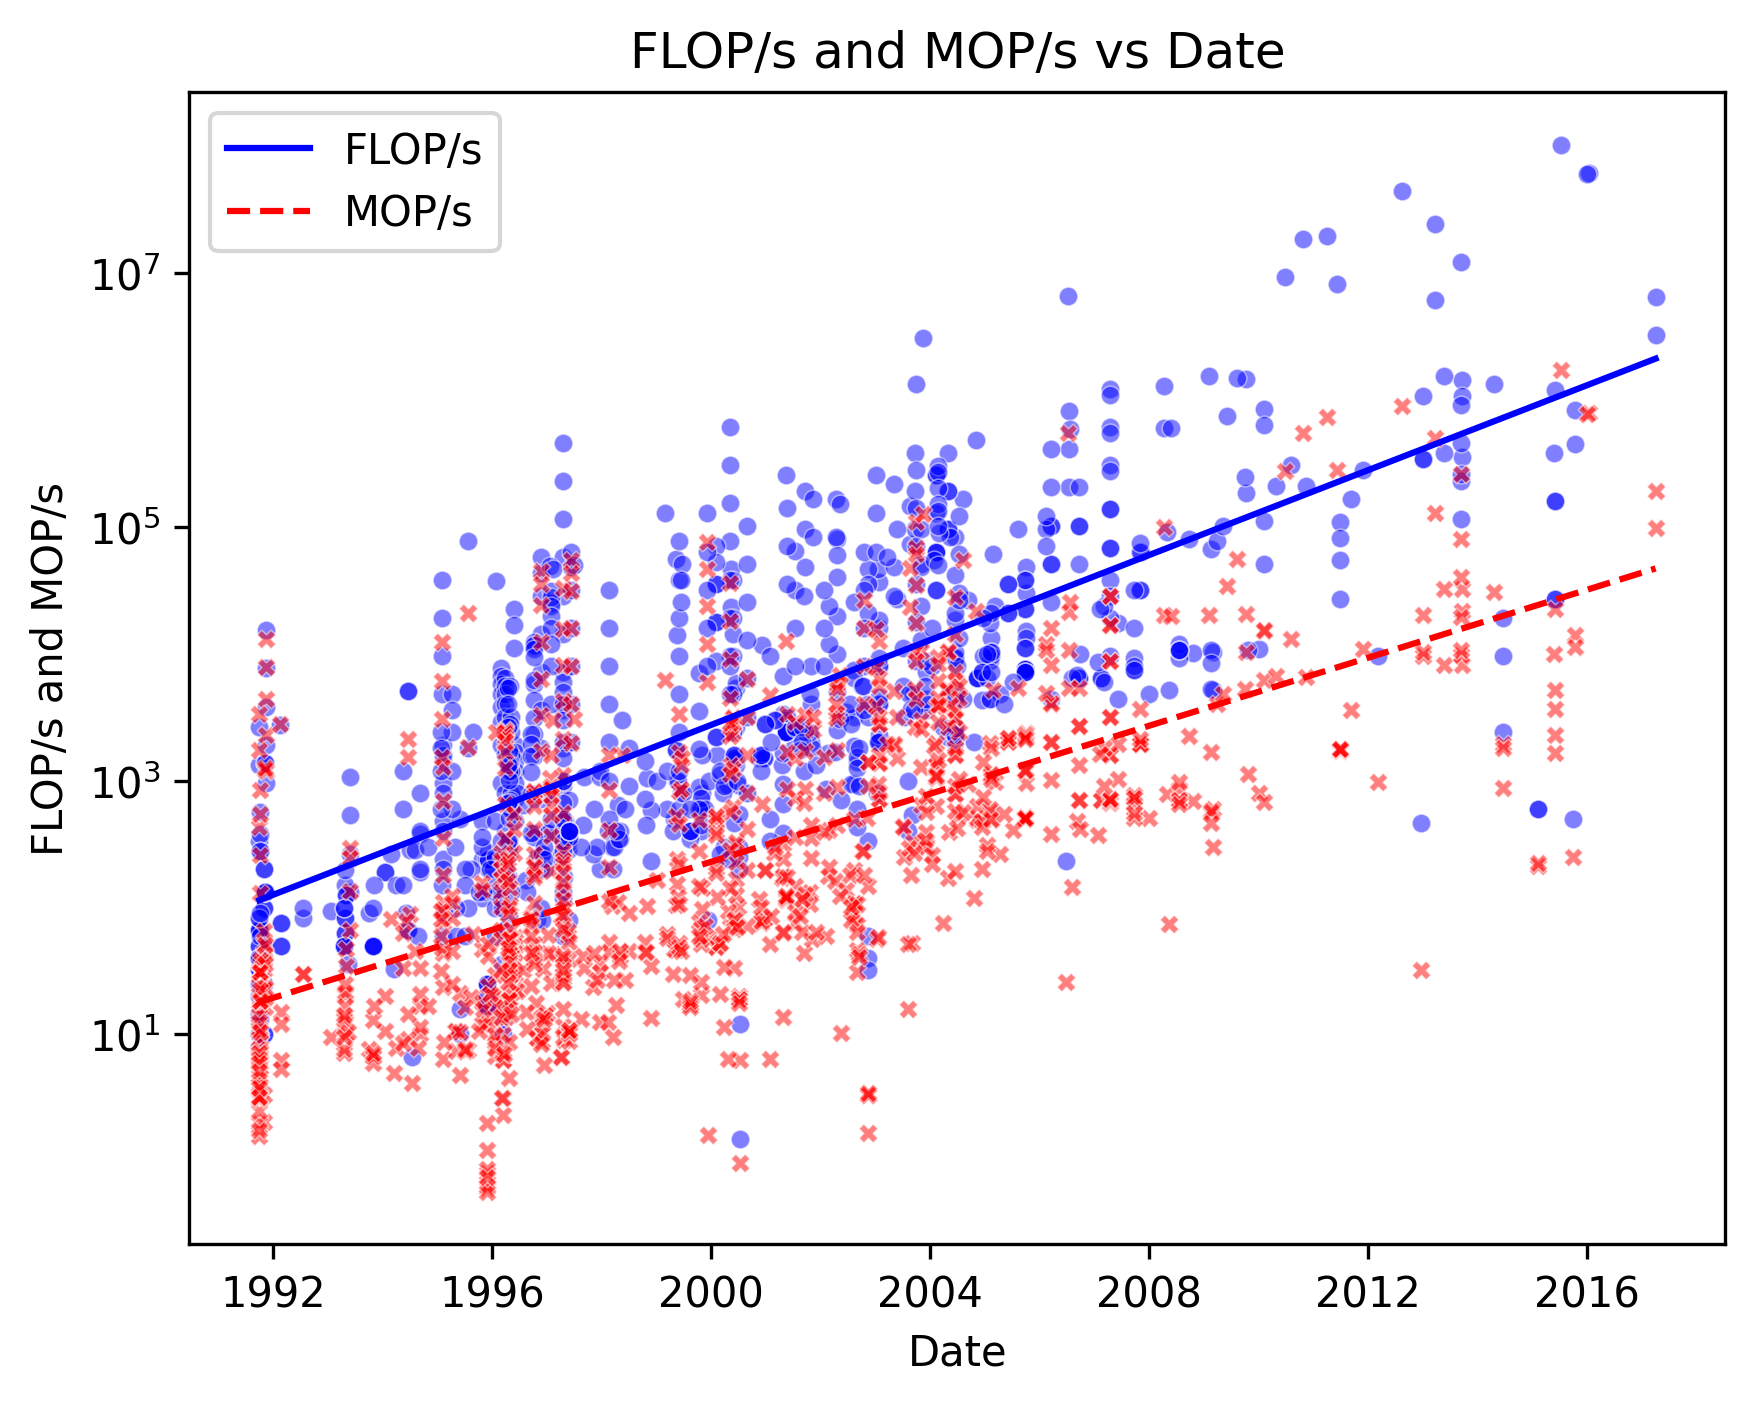
\includegraphics[width=\linewidth]{pictures/FLOPs_MOPs_vs_Date.png}
	\end{subfigure}
	\begin{subfigure}{.5\textwidth}
		\centering
		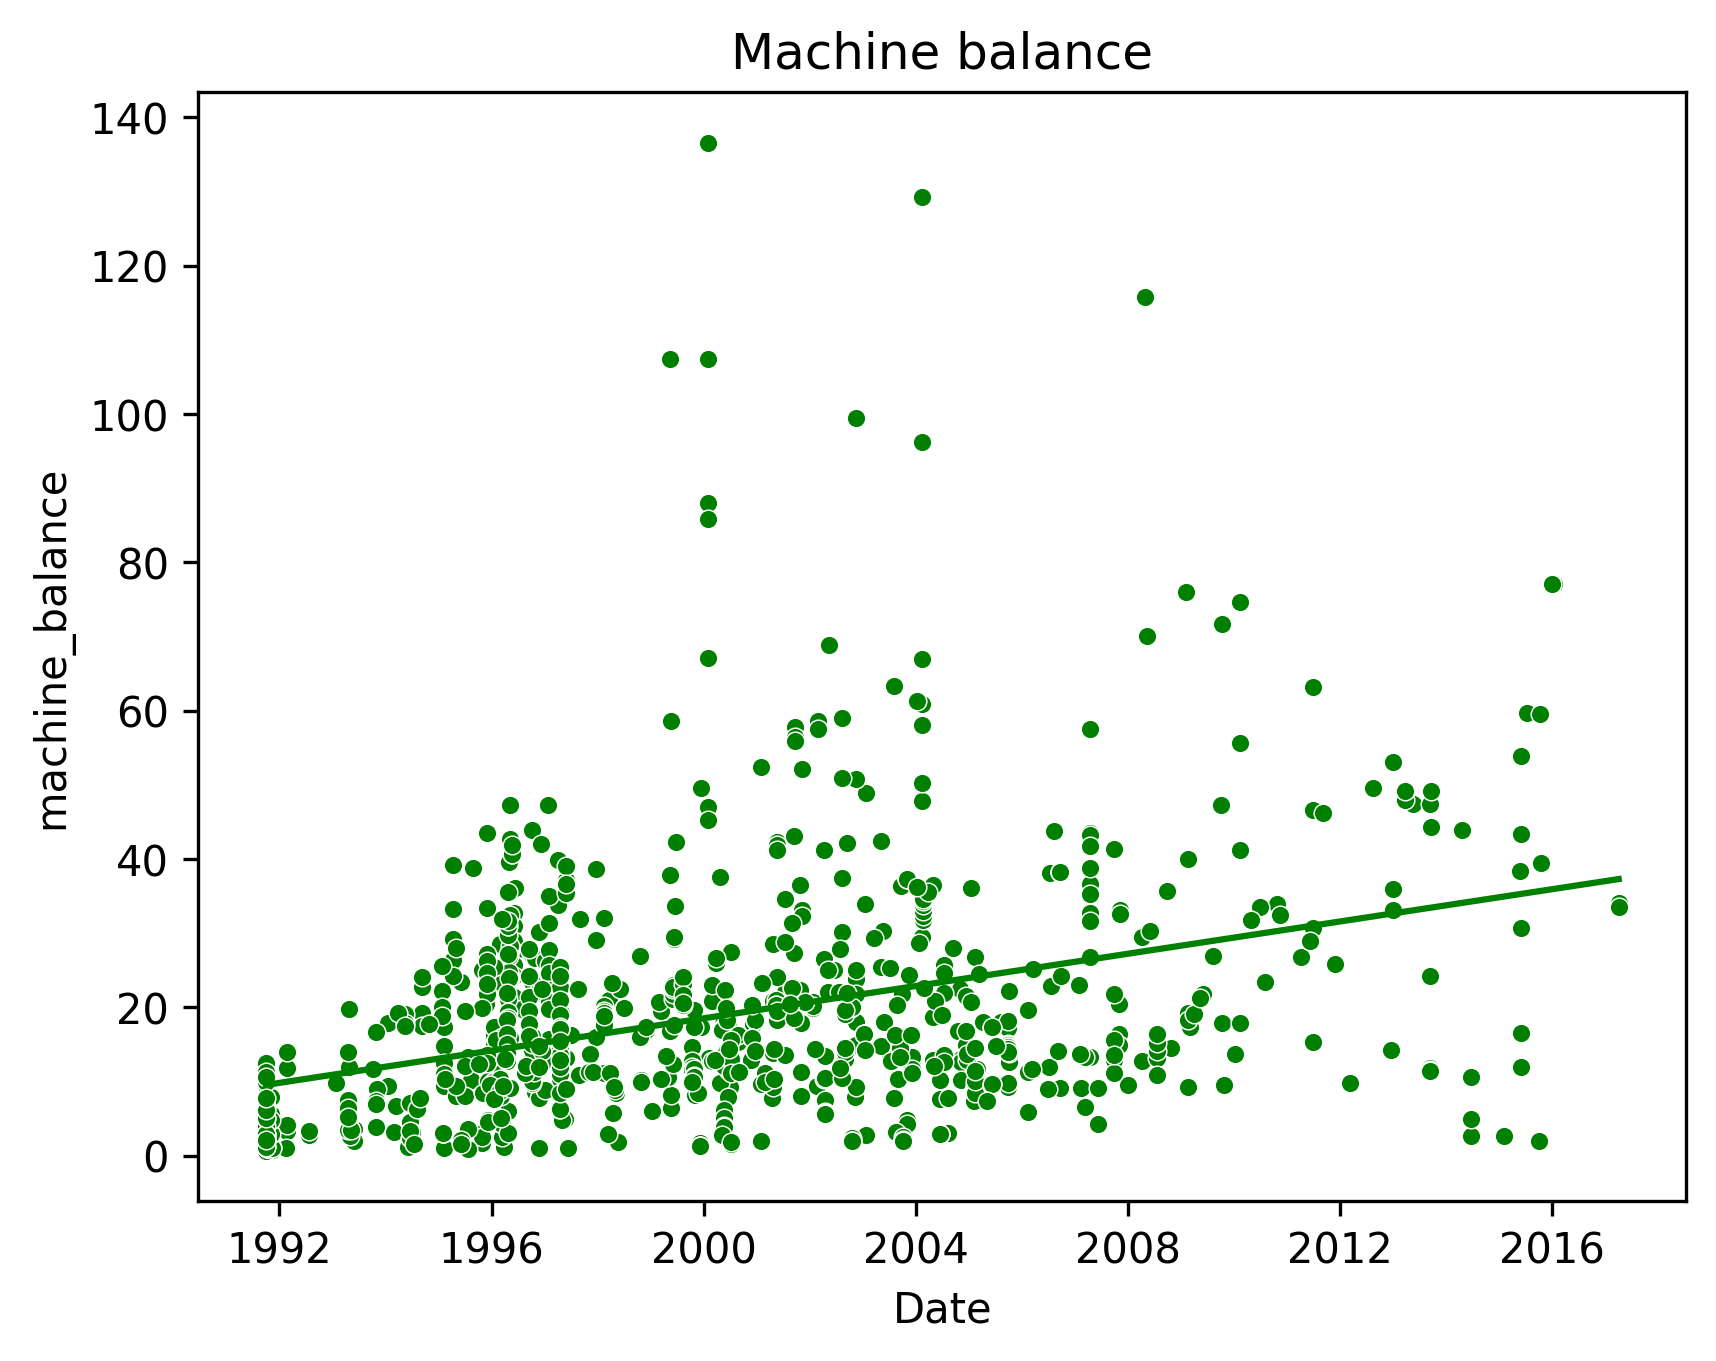
\includegraphics[width=\linewidth]{pictures/machine_balance.png}
	\end{subfigure}
	\caption{Illustration of the expanding processor-memory gap. The left graph charts the progression of FLOPs and MOPs on a logarithmic scale across various computing platforms, with the FLOPs trendline demonstrating a steeper ascent, indicative of the widening gap. The right figure depicts the development of the machine balance score for these platforms.\protect\footnotemark{}}
	\label{fig:pmgap}
\end{figure*}

The rest of the paper is structured as follows: Section \ref{sec:background} discusses the prevailing memory-related performance problems and their implications for modern computing systems. In Section \ref{sec:methods}, we delve into the various methods of acquiring memory-related performance data, with a focus on dynamic analysis, static analysis, and cache simulation. Section \ref{sec:visualization} provides a comprehensive overview of different visualization techniques used to interpret this data, while Section \ref{sec:optimization_workflow} outlines the standard workflow adopted by performance engineers to identify and mitigate memory-related bottlenecks. Section \ref{sec:works} presents an in-depth examination of exemplary memory access visualization tools, highlighting their unique strengths, weaknesses, and data gathering methods. Finally, the paper concludes with a discussion on the outlook for future work and potential improvements in this vital and rapidly-evolving field.